\documentclass[tikz,border=8pt]{standalone}
\usepackage{amsmath}
\usetikzlibrary{arrows.meta,positioning,fit}

\begin{document}
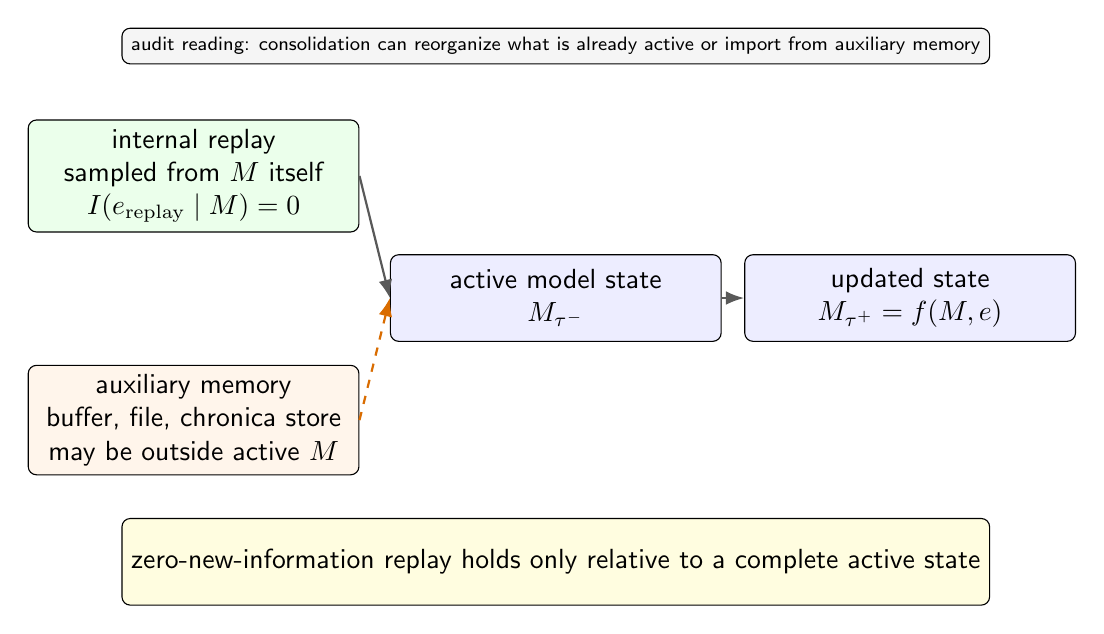
\begin{tikzpicture}[
  font=\sffamily,
  box/.style={draw, rounded corners=3pt, align=center, minimum width=42mm, minimum height=11mm, fill=white},
  note/.style={align=center, font=\sffamily\scriptsize},
  arrow/.style={-Latex, thick, draw=black!65},
  warn/.style={-Latex, thick, dashed, draw=orange!85!black}
]

\node[box, fill=blue!7] (m) at (4.6,0)
  {active model state\\$M_{\tau^-}$};
\node[box, fill=green!8] (internal) at (0,1.55)
  {internal replay\\sampled from $M$ itself\\$I(e_{\rm replay}\mid M)=0$};
\node[box, fill=orange!8] (archive) at (0,-1.55)
  {auxiliary memory\\buffer, file, chronica store\\may be outside active $M$};

\node[box, fill=blue!7] (m2) at (9.1,0)
  {updated state\\$M_{\tau^+}=f(M,e)$};

\draw[arrow] (internal.east) -- (m.west);
\draw[warn] (archive.east) -- (m.west);
\draw[arrow] (m.east) -- (m2.west);

\node[box, fill=yellow!12, minimum width=82mm] at (4.6,-3.35)
  {zero-new-information replay holds only relative to a complete active state};

\node[note, fill=gray!8, draw, rounded corners=3pt, minimum width=90mm] at (4.6,3.2)
  {audit reading: consolidation can reorganize what is already active or import from auxiliary memory};

\end{tikzpicture}
\end{document}
